\chapter{A Hybrid AI Architecture for Research Collaboration}\label{chap:Knowledge-DrivenArchitecture}
This chapter presents the architecture of the research collaboration recommender system, which is based on a hybrid \gls{ai} approach.
First of all, the ontology selection process, its description and some examples of subgraphs, are described in Sec.~\ref{sec:ontology-selection}.
Then, the recommendation strategy for suggesting both potential collaborators and the creation of consortia, is presented in Sec.~\ref{sec:recommendation-strategy}.
Finally, a comprehensive description of the system's architecture design is detailed in Sec.~\ref{sec:architecture-design}.
%
\section{Ontology Selection}\label{sec:ontology-selection}
In the problem awareness phase, we addressed the first sub-research question:
\begin{center}
    \rqOne
\end{center}
To establish a foundation for this study, we conducted a comprehensive literature review covering key areas such as research collaboration (Sec.~\ref{sec:research-collaboration}), the role of \acrlongpl{kg} and ontologies in the research domain (Sec.\ref{sec:knowledge-graphs}), \acrlongpl{llm} and their applications (Sec.~\ref{sec:large-language-models}), \acrlongpl{rag} concepts and approaches (Sec.~\ref{sec:retrieval-augmented-generation}), recommender systems tailored for research contexts (Sec.~\ref{sec:recommender-systems-in-research-field}), and the emerging field of Retrieval-Augmented Recommender Systems (Sec.~\ref{sec:retrieval-augmented-recommender-systems-in-research-field}).
From the literature review conducted, existing \glspl{kg} in the research field, such as \gls{mag}, \gls{s2ag}, Wikidata, \gls{orkg}, and VIVO ontology, were analyzed.
However, these \glspl{kg} and ontologies, present several limitations that impact their effectiveness in research collaborator recommendation such as:
\begin{itemize}
    \item Lack of granular and up-to-date data: many of these \glspl{kg} rely on static datasets or periodic updates, making it challenging to capture evolving research trends, emerging collaborations, and newly published work in real time.
    \item Limited contextual understanding: while these \glspl{kg} store structured information about authors, affiliations, and citations, they often lack deeper semantic connections, such as researchers' interdisciplinary expertise, project alignments, or implicit collaboration potential.
    \item Explainability and interpretability issues: many existing \glspl{kg} focus on metadata-level relationships rather than explaining why certain collaborations might be beneficial. This limits their ability to support explainable \gls{ai}-driven recommendations.
    \item Integration challenges: despite leveraging \gls{lod} principles, these \glspl{kg} are often designed with distinct schemas and ontologies, leading to interoperability challenges when combining multiple sources for enriched recommendations.
\end{itemize}

Given these limitations, the \gls{eurio} \gls{kg} was identified as particularly suitable for modeling European projects, making it an excellent choice for this thesis.
\gls{eurio} provides structured, rich metadata on European-funded projects, including participants, topics, and collaborations.
By leveraging \gls{eurio}, this thesis aims to overcome the limitations of existing \glspl{kg}, enabling a more dynamic, explainable, and semantically enriched recommendation framework.
The \gls{eurio} ontology and \gls{kg} are described in the following subsections.

Moreover, we found that most of the papers analyzed on recommender systems in the research domain, are designed to suggest research papers or to recommend collaborators.
In both cases, the most relevant aspects on which the recommender algorithms are based are influences on the number of citations, and abstracts of the papers.
Despite their advancements, recommender systems face significant limitations, particularly in complex domains like research collaboration.
Traditional methods such as \gls{cbf} and \gls{cf} suffer from data sparsity, making accurate recommendations difficult when user interaction data is limited.
The cold-start problem further complicates this by preventing effective suggestions for new users or items.
Additionally, many systems lack explainability, reducing user trust and interpretability, especially in critical decision-making contexts.
Another challenge is the tendency to prioritize historical patterns over novel discoveries, restricting interdisciplinary connections.
These limitations underscore the need for knowledge-aware recommender systems that integrate domain-specific semantics, contextual understanding, and explainable \gls{ai} techniques to enhance recommendation quality, fairness, and effectiveness.
We will focus on the identified research gap, which is in the limitations of \gls{dl}-based recommendation systems in capturing users' preferences, handling diverse textual information, and providing explainable recommendations.
These models often struggle to generalize to unseen scenarios and lack interpretability, making them less effective for tasks that require complex reasoning, such as recommendations from research collaborators.

\subsection*{EURIO: EUropean Research Information Ontology}
The \gls{eurio} ontology, developed by the Publications Office of the European Union\footnote{\url{https://op.europa.eu/en/}}, is a data model which conceptualizes, formally encodes, and makes available in an open, structured, and machine-readable format data about research projects funded by the EU's framework programmes for research and innovation.
\gls{cordis}, as described in Sec.~\ref{sec:dataset}, is responsible for publishing the results of these projects, while \gls{eurio} provides a semantic model that enhances transparency, reusability, and accessibility.
\gls{eurio} is built on top of well-known ontologies and vocabularies to ensure interoperability and semantic richness.
These include:
\begin{itemize}
    \item \gls{dc}: used for metadata elements such as titles, descriptions, and identifiers.
    \item \gls{dcat}: an \gls{rdf} vocabulary designed to facilitate interoperability between data catalogs published on the Web.
    \item \gls{dingo}: an ontology expressly designed to provide an extensible interoperable framework for formally conceptualizing and expressing the relevant parts of the research/cultural landscape in relation to funding, such that they can easily be shared between different actors and platforms.
    \item \gls{fabio}: facilitates the description of bibliographic entities and their relationships.
    \item \gls{frapo}: an ontology for describing the administrative information of research projects, e.g., grant applications, funding bodies, project partners, etc.
    \item \gls{foaf}: defines relationships between people and organizations.
    \item \gls{skos}: facilitates controlled vocabularies and classification schemes.
\end{itemize}

The \gls{eurio} ontology also incorporates reference data, such as countries, funding schemes, types of action, the EuroSciVoc taxonomy, and the NUTS classification, to enhance the semantic representation of research information.
It leverages the \gls{owl} 2 to formally define the semantics of domain-specific terms used to describe \gls{cordis} entities (e.g., projects, organizations, etc.), their attributes (e.g., title, acronym, legal name, etc.), and their interrelations (e.g., the connection between a project and its participating organizations, etc.).

\gls{eurio} defines multiple classes representing different concepts such as projects, organizations, funding schemes, grants, publications, and roles, along with associated data properties and object properties that define their relationships.
Each class has a set of data properties that describe its attributes, and a set of object properties that define its connections to other classes.
Each class, data property, and object property has several annotations but in general the main annotations for those are \textit{rdfs:label}, which provides a human-readable label for the entity, \textit{rdfs:comment}, which provides a human-readable description of the entity, and \textit{rdfs:isDefinedBy}, which provides a link to the ontology where the entity is defined.

For example, the title, description, start date, end date, and funding amount are data properties of the \textbf{Project} class.
The ontology also defines relationships between classes, such as \textbf{is funded by}, the association between a project and its grant (Fig.~\ref{fig:is-funded-by}).

\begin{figure}[htbp]
    \centering
 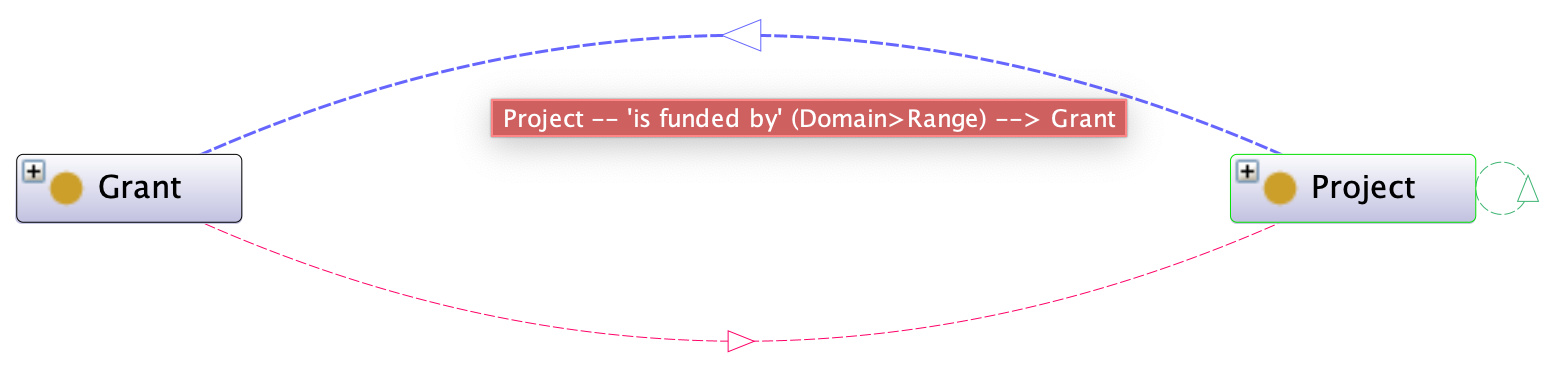
\includegraphics[width=.9\textwidth]{figures/architecture/is-funded-by.png}
     \rule{35em}{0.5pt}
    \caption{The ``is funded by'' relationship between a project and its grant}
 \label{fig:is-funded-by}
\end{figure}

Another example or relationship is \textbf{is employed by}, which links a person, in particular a \textbf{Person Role} to an \text{Organisation}.
The ontology also provides object property descrptions, for example the \textbf{has involved party} relationship, which links a \textbf{Project} to a \textbf{Role}, is inverse of \textbf{is involved in}, which links a \textbf{Role} to a \textbf{Project} (Fig.~\ref{fig:is-involved-in-has-involved-party}).

\begin{figure}[htbp]
    \centering
 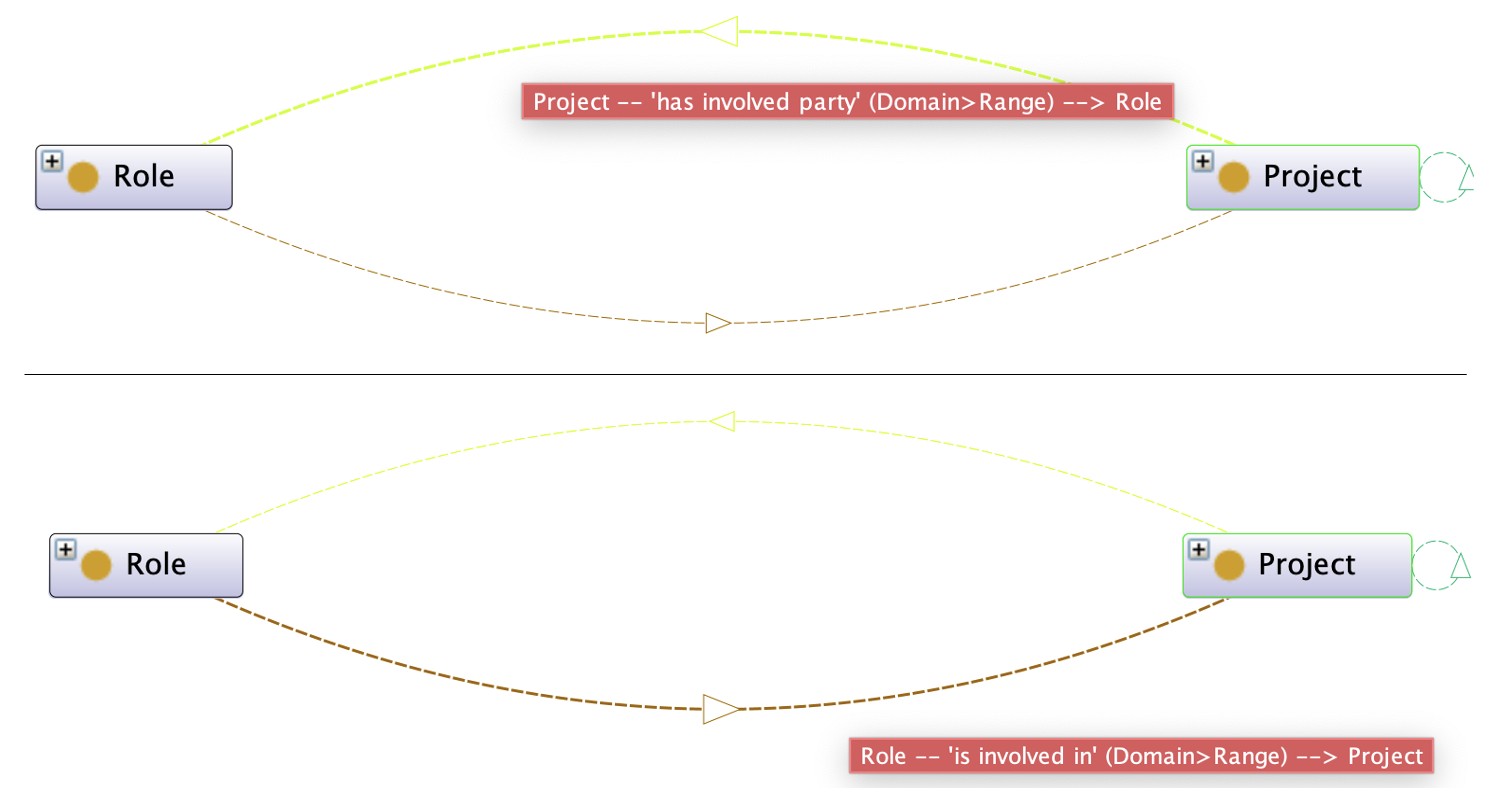
\includegraphics[width=.9\textwidth]{figures/architecture/has-involved-party-is-involved-in.png}
     \rule{35em}{0.5pt}
    \caption{The ``has involved party'' and ``is involved in'' relationships}
 \label{fig:is-involved-in-has-involved-party}
\end{figure}
\newpage
This object property descriptions can be very useful for querying the \gls{kg} to extract relevant information in a structured manner.
Moreover, the ontology defines a hierarchy of classes.
For example, the \textbf{Organisation} class is a superclass of several subclasses such as \textbf{For Profit Organisation}, \textbf{Funding Agency}, \textbf{Higher Or Secondary Education}, \textbf{Research Organisation}, and \textbf{SME} (Small and Medium Enterprise) (Fig.~\ref{fig:organisation-class-hierarchy}).

\begin{figure}[htbp]
    \centering
 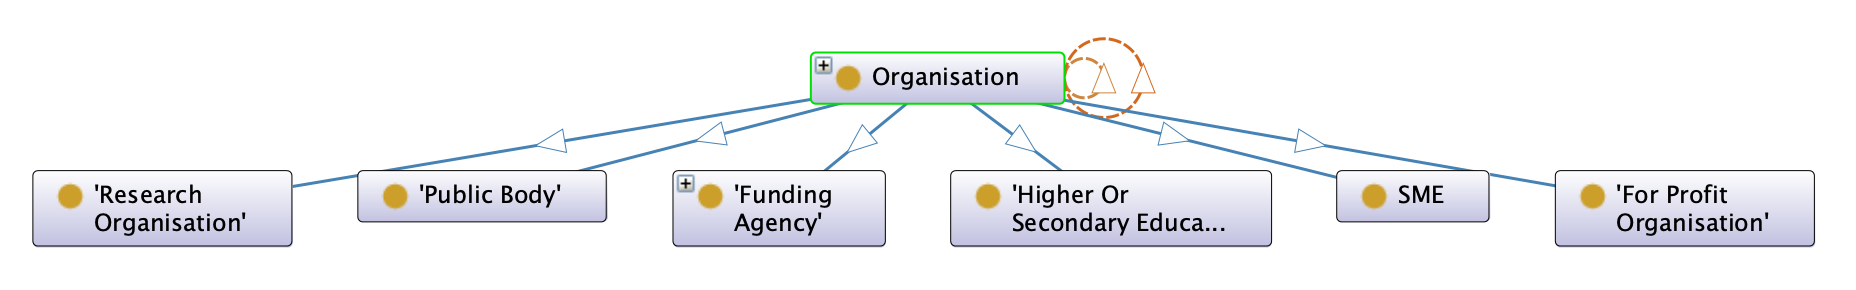
\includegraphics[width=.9\textwidth]{figures/architecture/organisation-class-hierarchy.png}
     \rule{35em}{0.5pt}
    \caption{The ``Organisation'' class hierarchy}
 \label{fig:organisation-class-hierarchy}
\end{figure}

An overview of the \gls{eurio} ontology is shown in the UML diagram in Fig.~\ref{fig:eurio-ontology}.

\begin{figure}[htbp]
    \centering
 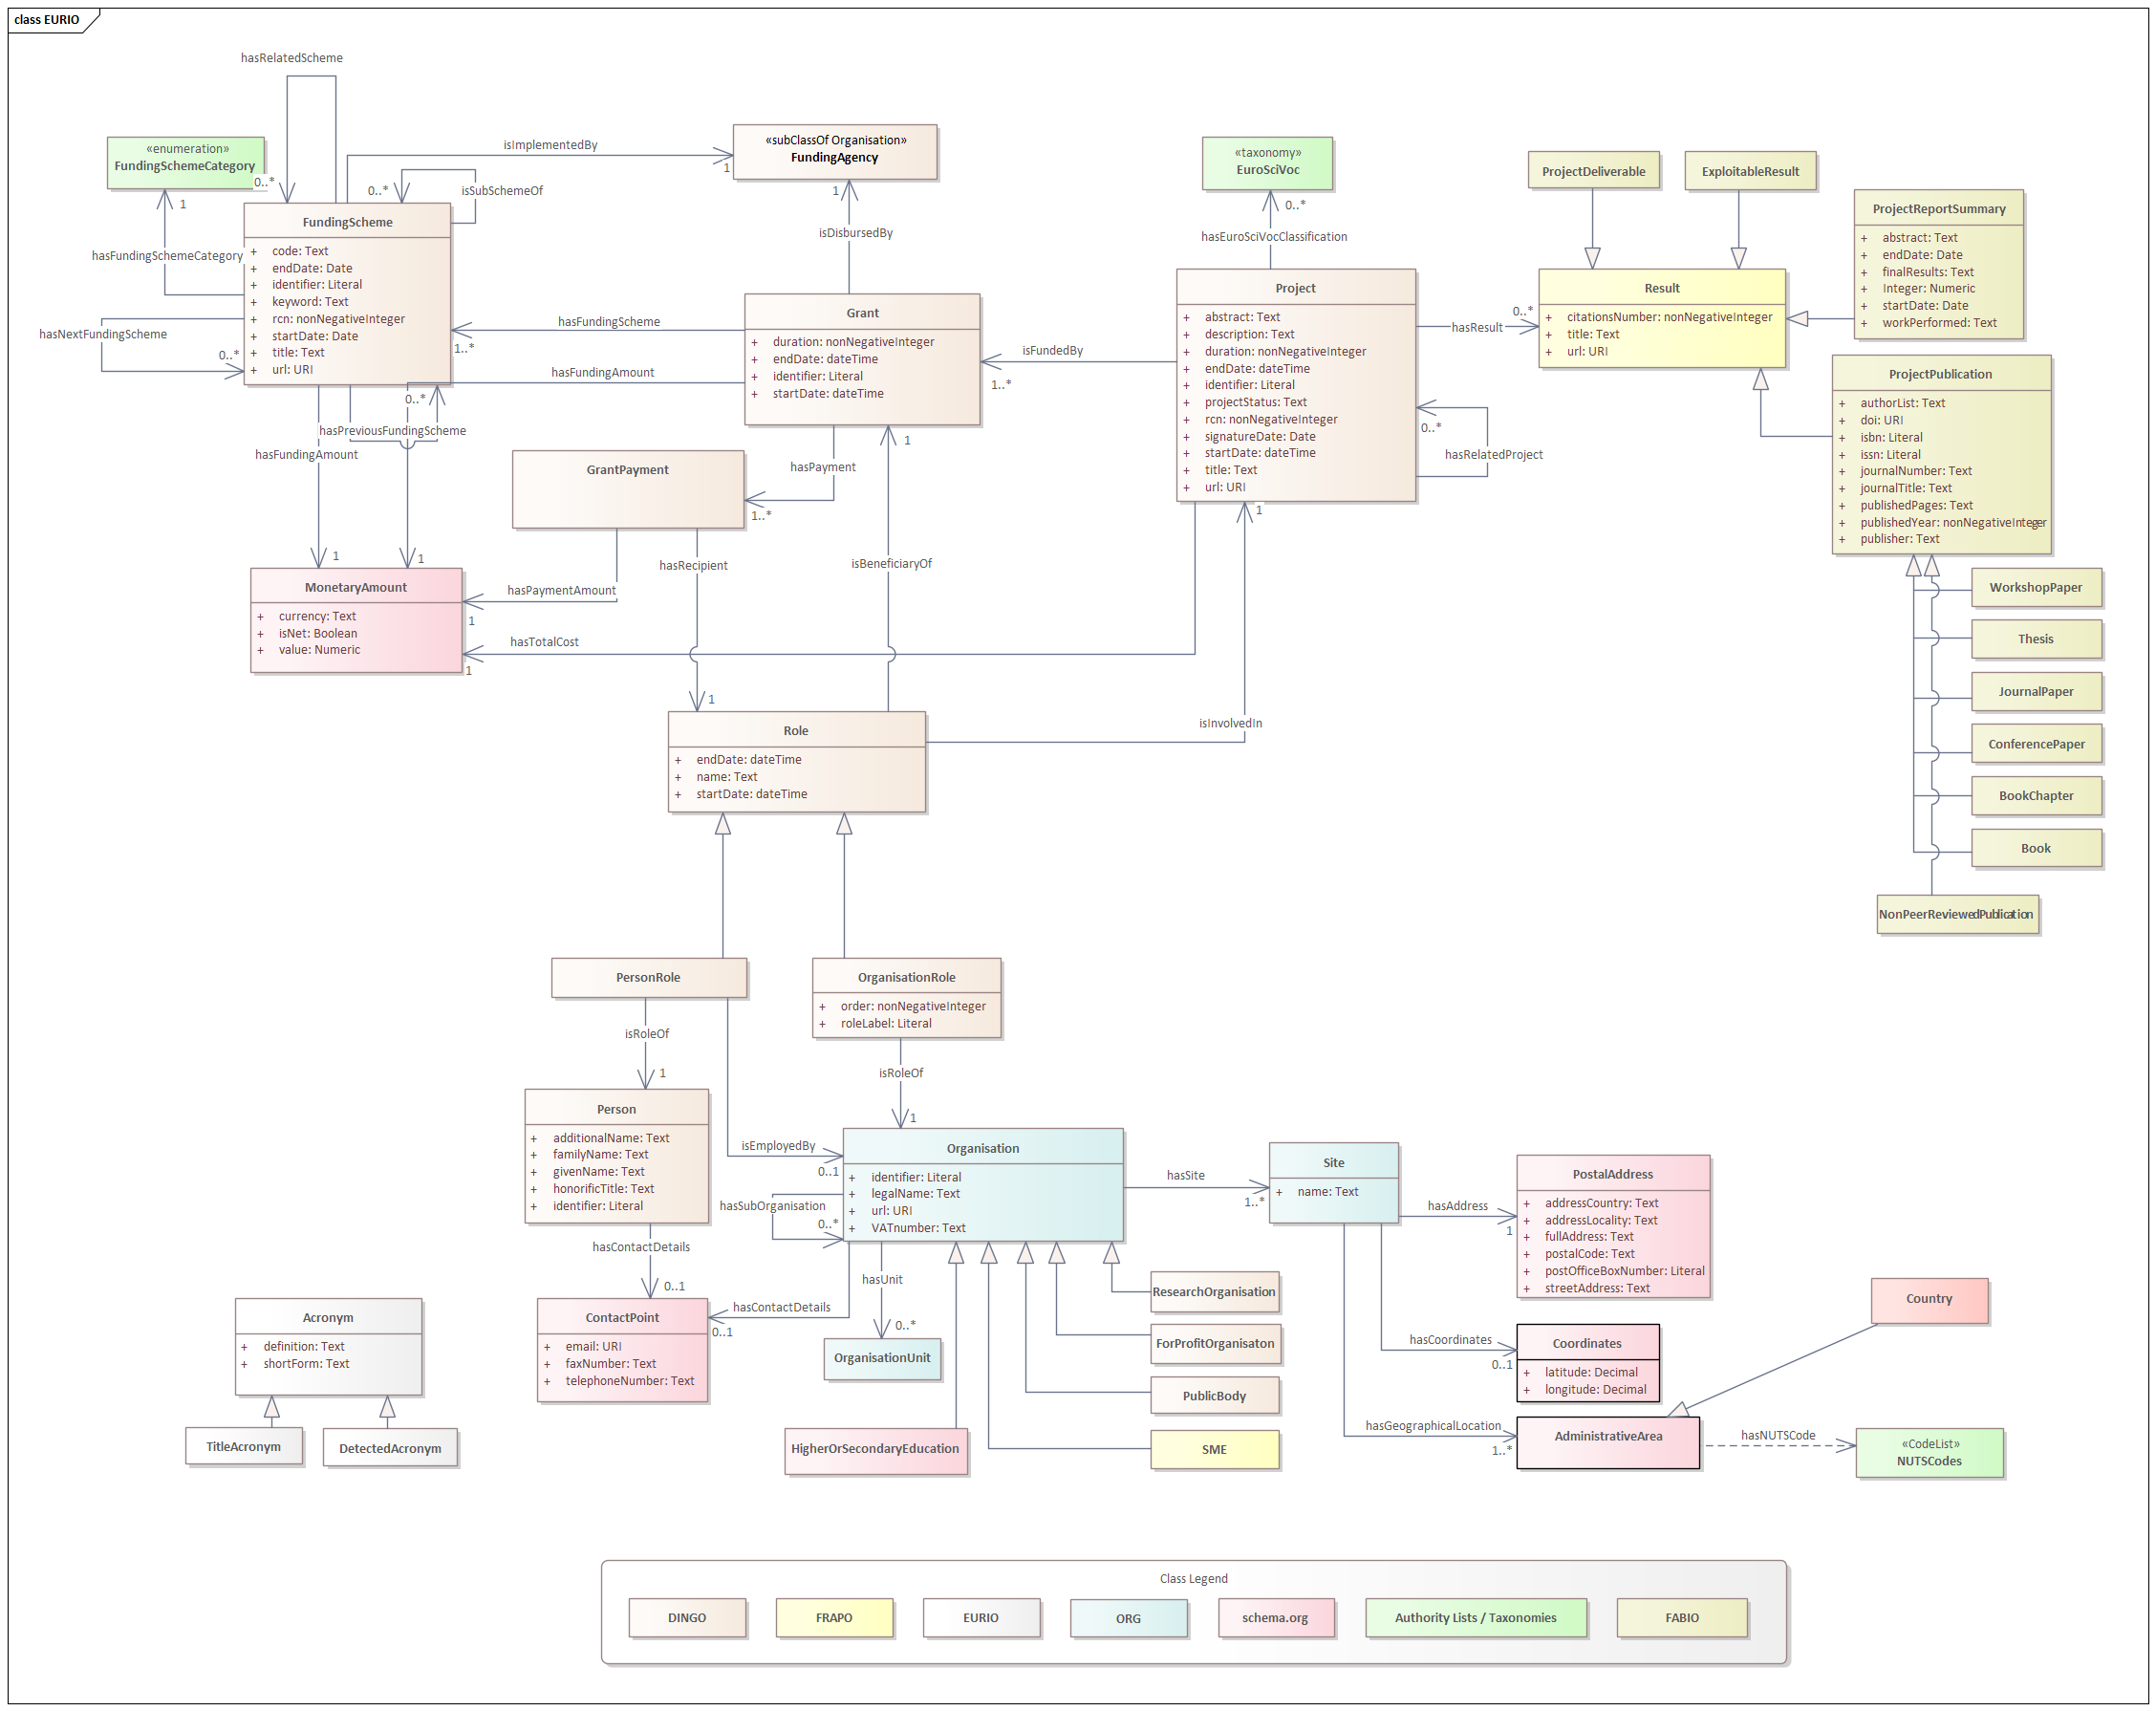
\includegraphics[width=\textwidth]{figures/architecture/EURIO_V2.4.png}
     \rule{35em}{0.5pt}
    \caption{A graphical representation of the \gls{eurio} ontology (from \url{https://op.europa.eu/en/web/eu-vocabularies/eurio})}
 \label{fig:eurio-ontology}
\end{figure}
\newpage

\subsection*{Data Availability and Formats}
The dataset is structured in \gls{rdf} format and contains over 18 million \gls{rdf} triples, with a total size of approximately 5GB when serialized in the N-Quad Triples \gls{rdf} format.
These structured triples enable the representation of relationships between projects, organizations, researchers, project publications, funding schemes, grants, countries, and other relevant entities making, the dataset a rich resource for \gls{kg}-based research.

The \gls{eurio} \gls{kg} is available in multiple formats to ensure accessibility and ease of integration into different research workflows.
Supported formats include \gls{rdf}, \gls{ttl}, \gls{nq}, \gls{jsonld}, and \gls{nt}.
The \gls{eurio} \gls{kg} used in this thesis is the latest version updated by the European Union on 08.11.2023, ensuring that the data remains relevant and accurate up to this date.

\section*{Knowledge Graph Exploration}
As previously explained, the \gls{eurio} \acrlong{kg} \cite{CORDIS_EURIO_2022} is built upon \gls{cordis} data and serves as a structured \gls{kg} that encapsulates information about research projects funded under the \gls{fp7} and \gls{h2020} framework programmes.
The \gls{eurio} \gls{kg} can be accessed via a \gls{sparql} endpoint at \url{https://cordis.europa.eu/datalab/sparql-endpoint/en}.
The \gls{kg} provides both database dumps and subsets of \gls{eurio} data in the form of named graphs.
The structure and organization of these named graphs are defined by the \gls{eurio} ontology, which is publicly available at: \url{https://op.europa.eu/en/web/eu-vocabularies/eurio}.

As part of this study, we conducted an exploration of the \gls{eurio} \gls{kg}, focusing on analyzing and understanding its ontology schema by identifying and examining the most important concepts, relationships, and structural elements.
This initial exploration allowed us to gain insights into the way projects, organizations, researchers, and related entities are modeled within the dataset.
For example, the Fachhochschule Nordwestschweiz and University of Camerino  subgraphs were extracted from the \gls{eurio} \gls{kg} to understand their properties and relationships.
Figures~\ref{fig:fhnw-graphdb} and~\ref{fig:unicam-graphdb} show the subgraphs for Fachhochschule Nordwestschweiz and University of Camerino, respectively, highlighting the connections between other entities.

\begin{figure}[htbp]
    \centering
 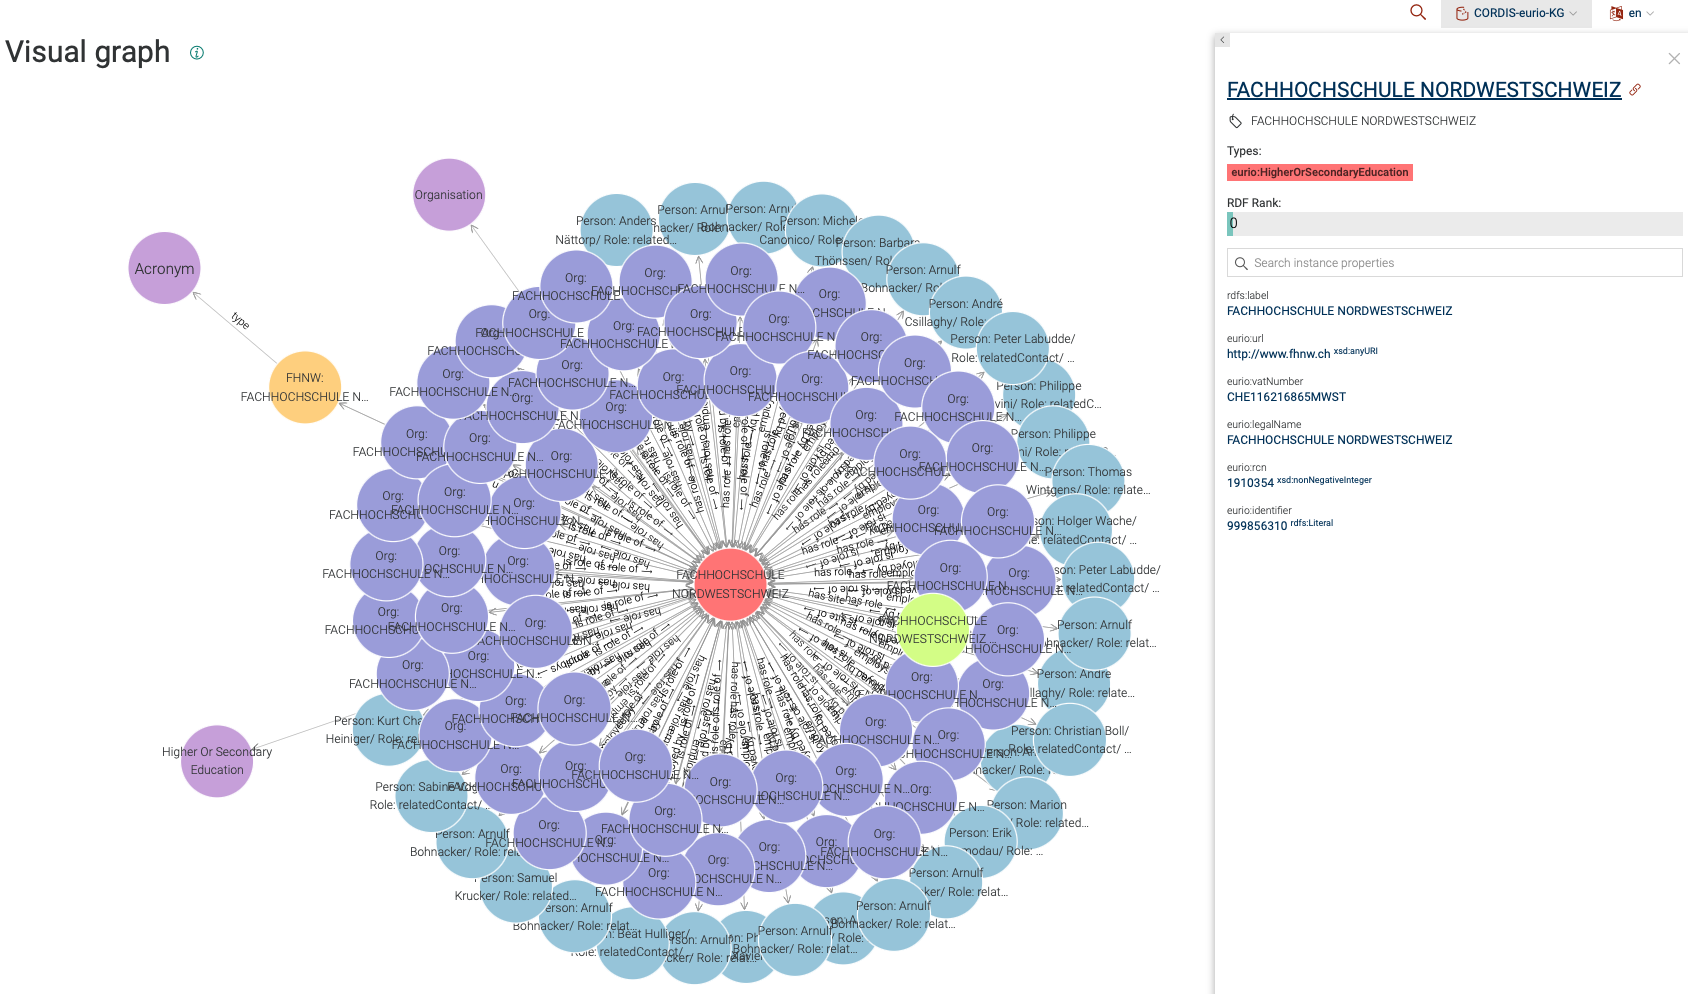
\includegraphics[width=.9\textwidth]{figures/architecture/graphdb-fhnw.png}
     \rule{35em}{0.5pt}
    \caption{FACHHOCHSCHULE NORDWESTSCHWEIZ subgraph in the \gls{eurio} \gls{kg}}
 \label{fig:fhnw-graphdb}
\end{figure}

\begin{figure}[htbp]
    \centering
 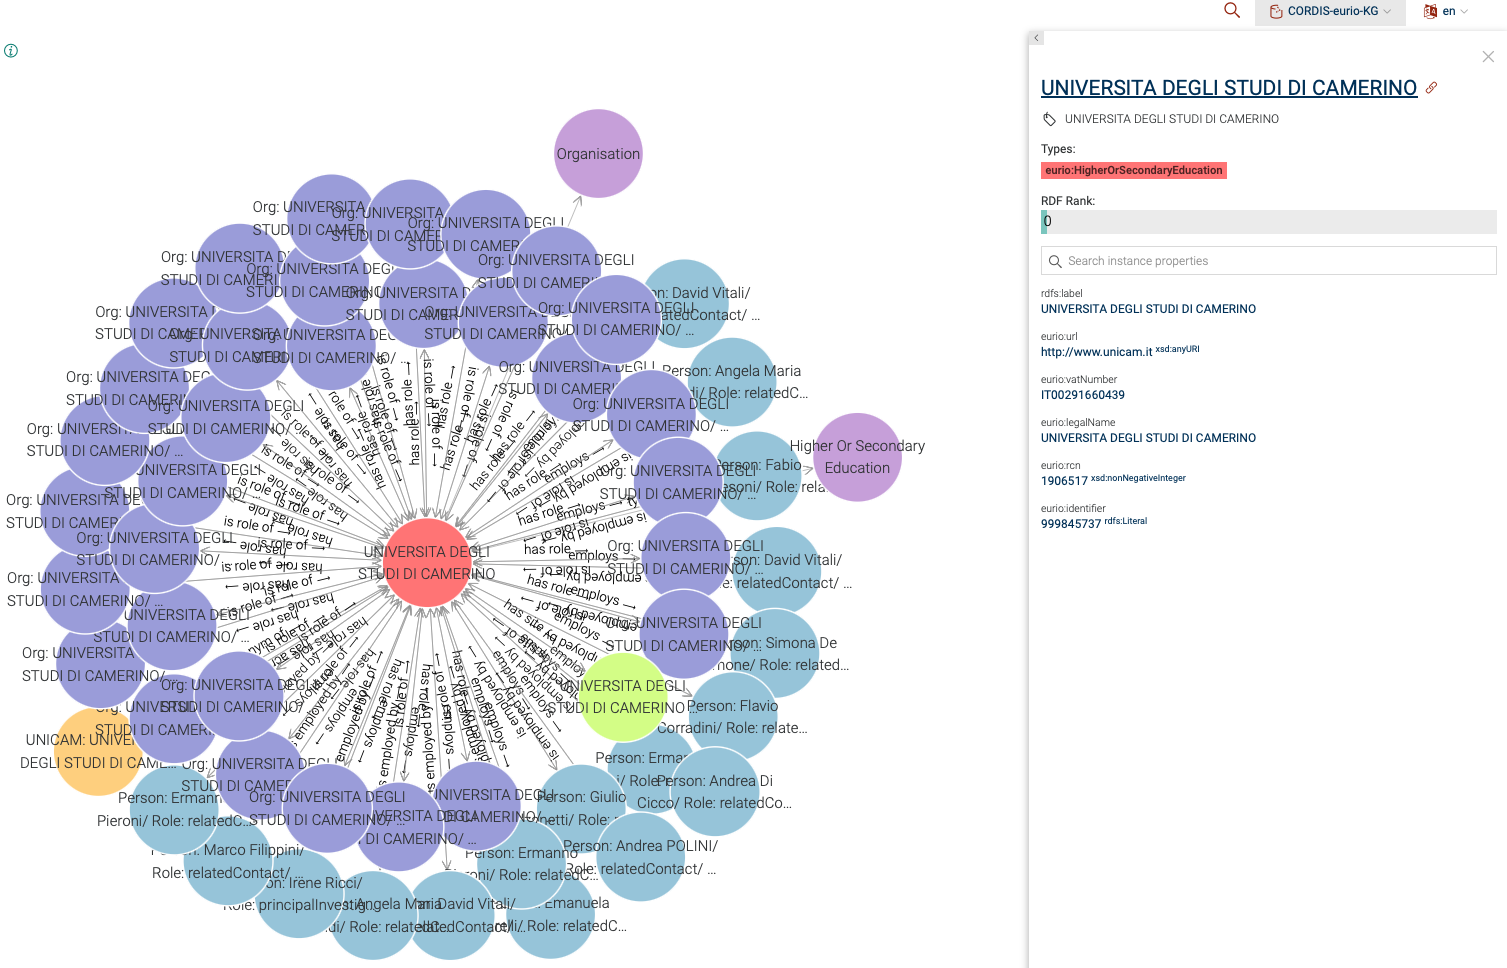
\includegraphics[width=.9\textwidth]{figures/architecture/graphdb-unicam.png}
     \rule{35em}{0.5pt}
    \caption{University of Camerino subgraph in the \gls{eurio} \gls{kg}}
 \label{fig:unicam-graphdb}
\end{figure}
\newpage
As can be seen from both figures, both the Fachhochschule Nordwestschweiz and the University of Camerino are instances of the \textbf{eurio:HigherOrSecondaryEducation} class and have the following six data properties: \textit{rdfs:label}, \textit{eurio:url}, \textit{eurio:vatNumber}, \textit{eurio:legalName}, \textit{eurio:rcn}, and \textit{eurio:identifier}.
Furthermore, we can see that, taking Fachhochschule Nordwestschweiz as an example, it has several \textit{eurio:hasRole} relationships with different ``Org: FACHHOCHSCHULE NORDWESTSCHWEIZ'' entities.
The \gls{kg} contains several such redundancies, also for other types of classes.
Each entity of type \textbf{eurio:Organisation} has several relationships with the entity of type \textbf{eurio:OrganisationRole}.
This type of relationship implies a lot of redundancy in the nodes of the \gls{kg}, but is deduced to be necessary to represent the project-related organisation role.
For example, as illustrated in Fig.~\ref{fig:fhnw-organisationRole-example}, the Fachhochschule Nordwestschweiz node is linked via the \textit{euro:hasRole} relationship, to the node ``Org: FACHHOCHSCHULE NORDWESTSCHWEIZ/ Role: participant/ Project: 53135'', which semantically represents the participation of the Fachhochschule Nordwestschweiz in the project with project ID 53135.
From the data properties of this node, we can easily see that the role of the FHNW in this project was participant, and that the project duration was from April 4, 2018, to September 30, 2021.

\begin{figure}[htbp]
    \centering
 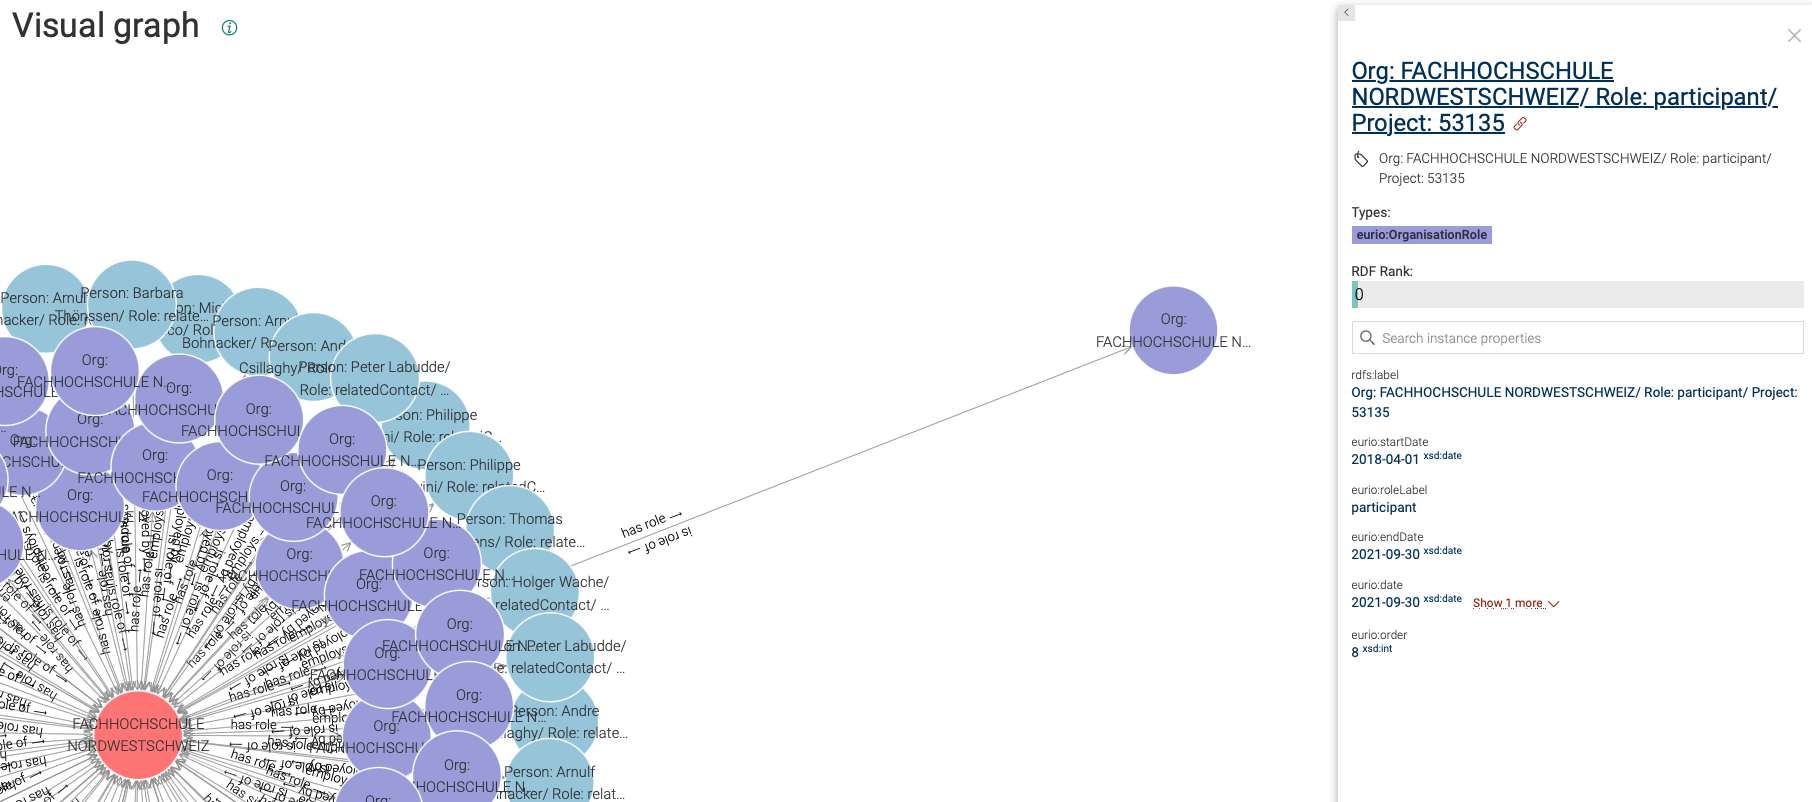
\includegraphics[width=.9\textwidth]{figures/architecture/graphdb-fhnw-organisationRole-example.png}
     \rule{35em}{0.5pt}
    \caption{An example of an OrganisationRole entity in the FHNW subgraph}
 \label{fig:fhnw-organisationRole-example}
\end{figure}

Following this, we performed a more in-depth exploration using \gls{sparql} queries to retrieve and analyze various aspects of the \gls{kg}.
This included examining the metadata of research projects, their abstract, start and end dates, project status, as well as the organizations involved, their roles, and the researchers affiliated with them.
For example, Listing~\ref{lst:sparql_example_project1_data_properties} shows a \gls{sparql} query that retrieves the abstract, status, start date, and end date of a specific project titled ``BIM-based holistic tools for Energy-driven Renovation of existing Residences'', which was selected as a scenario example (Project \ref{project1}) for this study in Sec.~\ref{sec:scenarios}.
The results of this query are shown in Fig.~\ref{fig:sparql_example_project1_data_properties}, providing detailed information about some project data properties.

\begin{lstlisting}[language=SPARQL, caption={\gls{sparql} query for getting the abstract, status, start date, and end date of a project titled ``BIM-based holistic tools for Energy-driven Renovation of existing Residences''}, label=lst:sparql_example_project1_data_properties]
    PREFIX eurio: <http://data.europa.eu/s66#>
    SELECT ?abstract ?status ?start_date ?end_date
    WHERE {
        ?project a eurio:Project ; 
            eurio:title "BIM-based holistic tools for Energy-driven Renovation of existing Residences" ;
            eurio:abstract ?abstract ;
            eurio:startDate ?start_date ;
            eurio:endDate ?end_date ;
            eurio:projectStatus ?status .
    }
\end{lstlisting}

\begin{figure}[htbp]
    \centering
 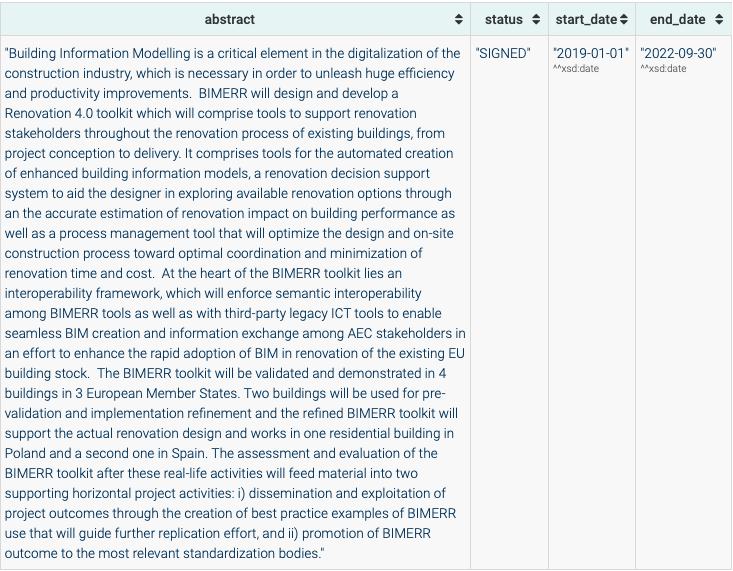
\includegraphics[width=.8\textwidth]{figures/architecture/sparql_example_project1_data_properties.png}
     \rule{35em}{0.5pt}
    \caption{\gls{sparql} query results for getting the abstract, status, start date, and end date of a project titled ``BIM-based holistic tools for Energy-driven Renovation of existing Residences''}
 \label{fig:sparql_example_project1_data_properties}
\end{figure}

We also explored the consortium participants involved in the selected project by querying the \gls{kg} to retrieve the organizations and their roles in the project.
Listing~\ref{lst:sparql_example_project1_consortium_participants} shows the \gls{sparql} query used to extract the consortium participants involved in the project \ref{project1}.
The results of this query are shown in Fig.~\ref{fig:sparql_example_project1_consortium_participants}, providing detailed information about the organizations and their roles in the project.
As we can see, the consortium participants are the same as the ones listed in the scenario analysis in Sec.~\ref{sec:scenarios}.

\begin{lstlisting}[language=SPARQL, caption={\gls{sparql} query for getting the consortium participants involved in a project titled ``BIM-based holistic tools for Energy-driven Renovation of existing Residences''}, label=lst:sparql_example_project1_consortium_participants]
    PREFIX eurio: <http://data.europa.eu/s66#>
    PREFIX rdfs: <http://www.w3.org/2000/01/rdf-schema#>
    SELECT DISTINCT (COALESCE(?org, STRBEFORE(STRAFTER(?party_title, "Org: "), "/ Role:")) AS ?organisation) ?role_label
    WHERE {
        ?project a eurio:Project .
        ?project eurio:title "BIM-based holistic tools for Energy-driven Renovation of existing Residences".
        ?project eurio:title ?project_title.
        ?project eurio:hasInvolvedParty ?party .
        ?party a eurio:OrganisationRole.
        ?party eurio:roleLabel ?role_label.
        ?party rdfs:label ?party_title.
        OPTIONAL { ?party eurio:isRoleOf ?role . ?role rdfs:label ?org. }
    }
\end{lstlisting}

\begin{figure}[htbp]
    \centering
 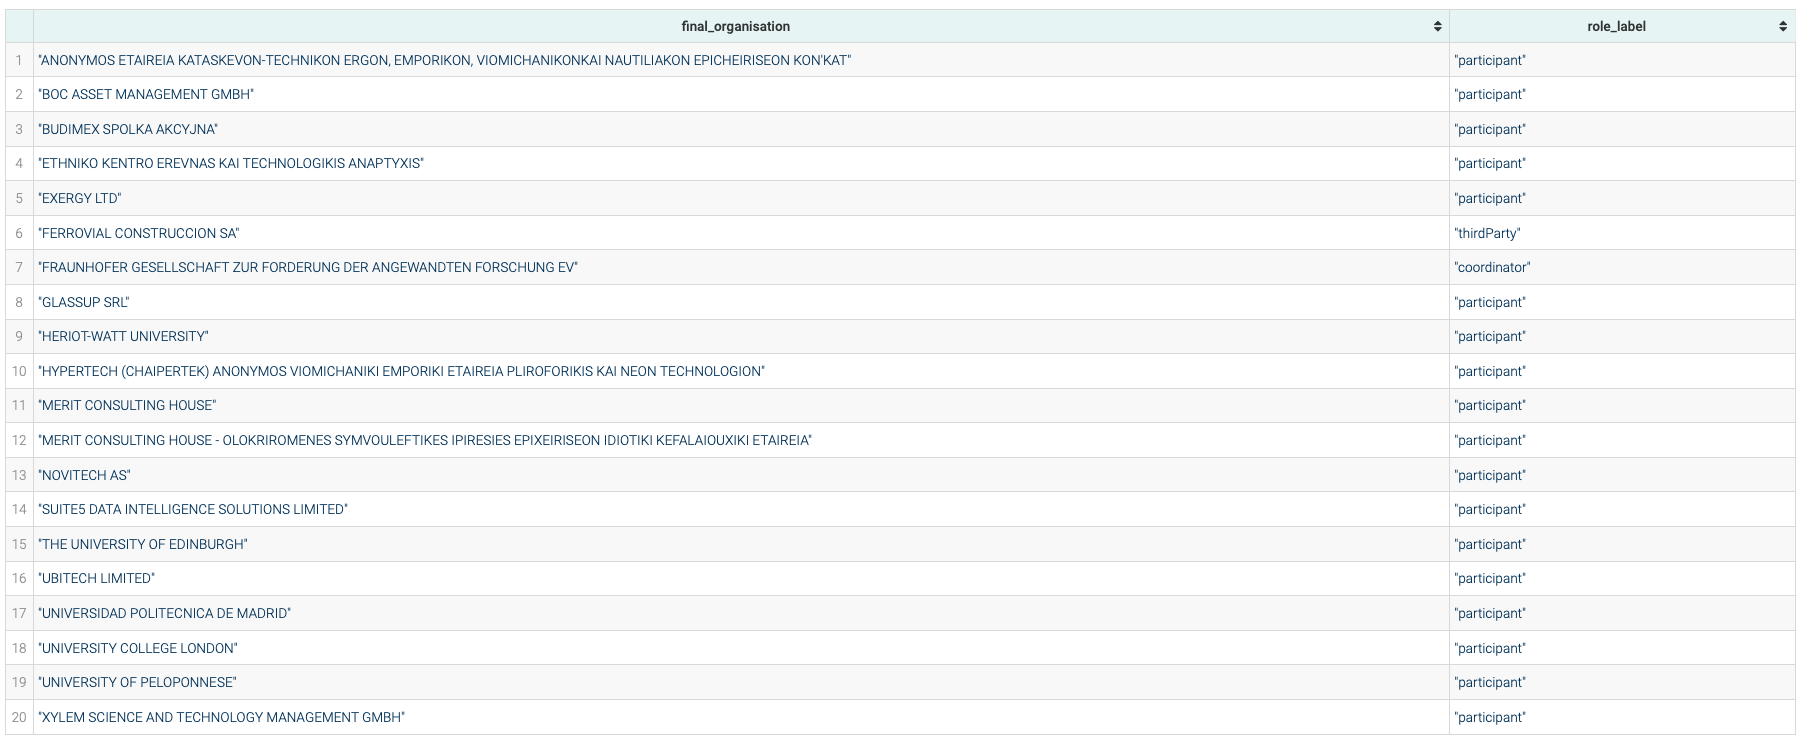
\includegraphics[width=.8\textwidth]{figures/architecture/sparql_example_project1_consortium_participants.png}
     \rule{35em}{0.5pt}
    \caption{\gls{sparql} query results for getting the consortium participants involved in a project titled ``BIM-based holistic tools for Energy-driven Renovation of existing Residences''}
 \label{fig:sparql_example_project1_consortium_participants}
\end{figure}

During the exploration, we also investigated people involved in research projects.
In the \gls{eurio} \gls{kg}, every project includes information about the organizations involved.
Unfortunately, not all projects have the \textit{eurio:isEmployedBy} relationship linking a \textbf{eurio:Role} to a \textbf{eurio:Organisation}.
As a result, it is not always possible to retrieve details about the individuals associated with a given project, since their employment or involvement is not explicitly represented in all cases.
The selected project \ref{project1}, is an example of a project where the people involved are not explicitly linked to the project.
Running the query in Listing~\ref{lst:sparql_example_project1_people} on the \gls{eurio} \gls{kg} did not return any results, indicating that the people involved in the project are not explicitly linked to the project.

\begin{lstlisting}[language=SPARQL, caption={\gls{sparql} query for getting full name, organisation, telephone, and fax of the people involved in a project titled ``BIM-based holistic tools for Energy-driven Renovation of existing Residences''}, label=lst:sparql_example_project1_people]
    PREFIX eurio: <http://data.europa.eu/s66#>
    PREFIX rdfs: <http://www.w3.org/2000/01/rdf-schema#>
    SELECT ?person_label ?org_name ?telephone ?fax
    WHERE {
        ?person a eurio:Person .
        ?person rdfs:label ?person_label .
        ?person eurio:hasContactDetails ?contact_details.
        ?contact_details eurio:telephone ?telephone.
        ?contact_details eurio:faxNumber ?fax.
        ?person eurio:hasRole ?role.
        ?role eurio:isEmployedBy ?org.
        ?org rdfs:label ?org_name.
        ?role eurio:isInvolvedIn ?project.
        ?project a eurio:Project.
        ?project eurio:title "BIM-based holistic tools for Energy-driven Renovation of existing Residences".
    }
\end{lstlisting}

Listing~\ref{lst:sparql_example_merelli_project_people} is the same query as Listing~\ref{lst:sparql_example_project1_people}, but for a different project titled ``Topology driven methods for complex systems''.
The results of this query are shown in Fig.~\ref{fig:sparql_example_merelli_project_people}, providing detailed information about the people involved in the project, including their full name, organization, telephone, and fax.

\begin{lstlisting}[language=SPARQL, caption={\gls{sparql} query for getting full name, organisation, telephone, and fax of the people involved in a project titled ``Topology driven methods for complex systems''}, label=lst:sparql_example_merelli_project_people]
    PREFIX eurio: <http://data.europa.eu/s66#>
    PREFIX rdfs: <http://www.w3.org/2000/01/rdf-schema#>
    SELECT ?person_label ?org_name ?telephone ?fax
    WHERE {
        ?person a eurio:Person .
        ?person rdfs:label ?person_label .
        ?person eurio:hasContactDetails ?contact_details.
        ?contact_details eurio:telephone ?telephone.
        ?contact_details eurio:faxNumber ?fax.
        ?person eurio:hasRole ?role.
        ?role eurio:isEmployedBy ?org.
        ?org rdfs:label ?org_name.
        ?role eurio:isInvolvedIn ?project.
        ?project a eurio:Project.
        ?project eurio:title "Topology driven methods for complex systems".}
\end{lstlisting}

\begin{figure}[htbp]
    \centering
 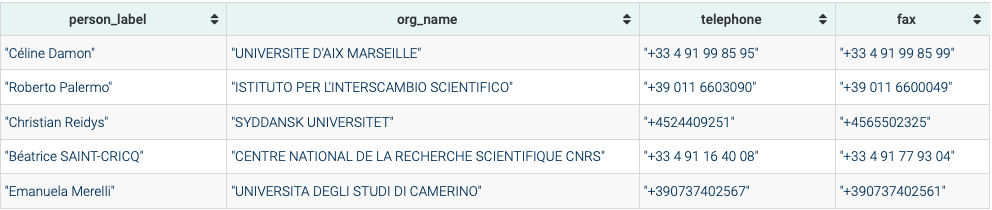
\includegraphics[width=.9\textwidth]{figures/architecture/sparql_example_merelli_project_people.png}
     \rule{35em}{0.5pt}
    \caption{\gls{sparql} query results for getting full name, organisation, telephone, and fax of the people involved in a project titled ``Topology driven methods for complex systems''}
 \label{fig:sparql_example_merelli_project_people}
\end{figure}

The last person in the results of the query in Listing~\ref{lst:sparql_example_merelli_project_people} is Prof. Emanuela Merelli, who is affiliated with the University of Camerino, and Fig.~\ref{fig:example-person-prof-merelli} presents a visual representation of the \gls{eurio} \gls{kg}, specifically focusing on her class type as a \textbf{eurio:Person}.

At the center of the graph, her node connects to multiple entities representing affiliations, roles, projects, and contact details.
The right panel provides metadata about her, including her given name, family name, research control number, and honorific title, indicating her academic status as ``Prof.''.
From Emanuela Merelli's node, one connection leads to a contact details node, which contains her telephone number (+390737402567) and fax number (+390737402561), establishing the \textit{eurio:hasContactDetails} relationship.

\begin{figure}[htbp]
    \centering
 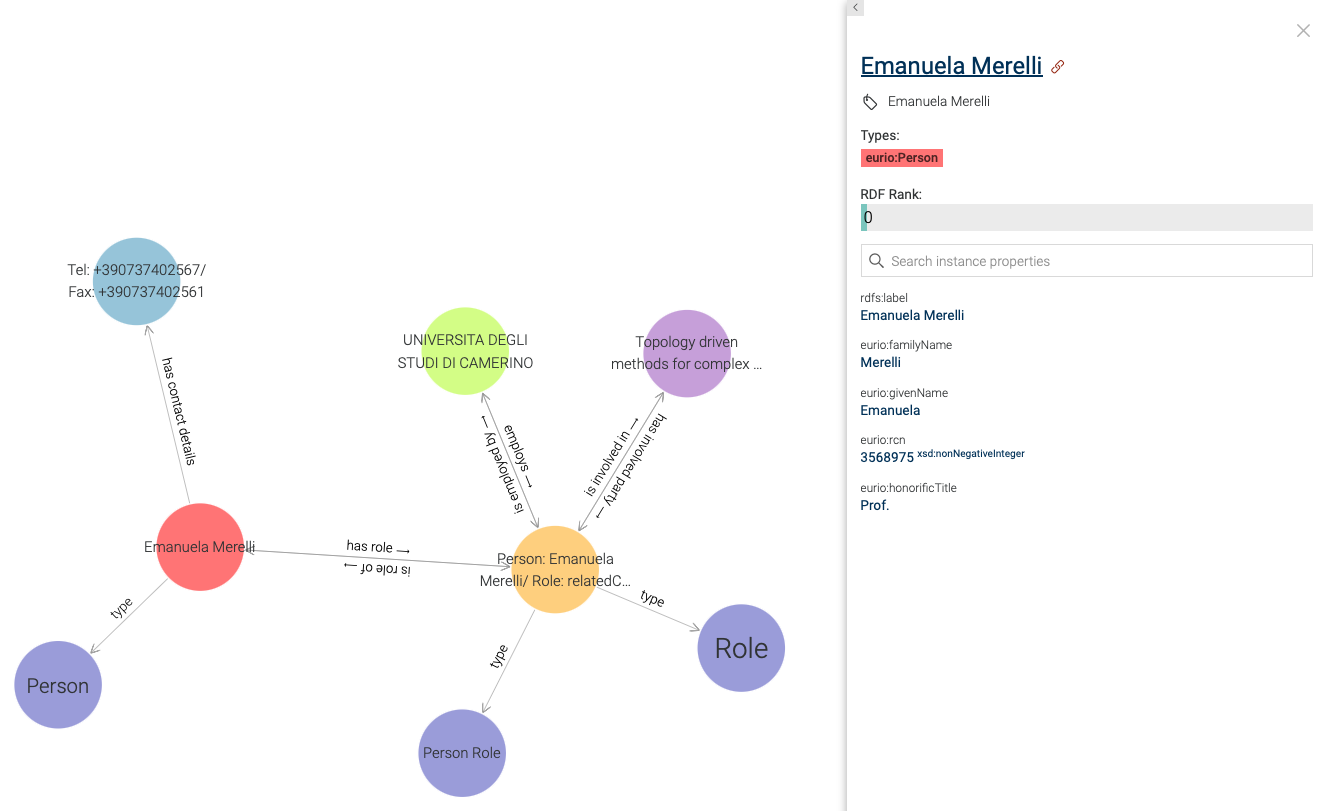
\includegraphics[width=.9\textwidth]{figures/architecture/example-person-prof-merelli.png}
     \rule{35em}{0.5pt}
    \caption{An example of a person's profile in the \gls{eurio} \gls{kg}}
 \label{fig:example-person-prof-merelli}
\end{figure}

Another key connection links her to the ``Universit\`a degli Studi di Camerino'', represented as a green node, with the \textit{eurio:isEmployedBy} relationship, signifying her affiliation with this institution.
Her professional involvement is further detailed through an orange node representing her role, which is bidirectionally linked to her node through the \textit{eurio:hasRole} and \textit{eurio:isRoleOf} relationships.
This \textbf{eurio:PersonRole} node serves as an intermediary between her and the projects she is involved in.
Another significant connection in the graph extends from the role node to a purple node, which is an instance of \textbf{eurio:Project} class, and represents a research project titled ``Topology driven methods for complex systems'', indicating her involvement.
The connection between the role and the project is represented by the \textit{eurio:isInvolvedIn} relationship, confirming her participation in the research activity.
Additional purple nodes represent the classification of roles, distinguishing between general role types and specific person roles.


Through this query-based investigation, we were able to extract detailed information on how projects are interconnected, how participants are structured, and how different elements contribute to the overall knowledge representation within \gls{eurio}.
This \gls{kg} exploration provided a comprehensive understanding of the dataset's richness and limitations, enabling a more informed approach in leveraging the \gls{kg} for our study.

Leveraging the \gls{eurio} ontology, we can effectively address the first sub-research question by structuring and representing data on researchers and research projects within a \gls{kg}.
%
\section{Recommendation Strategy}\label{sec:recommendation-strategy}


The recommendation strategy in this study was designed to leverage the structured data and relationships within the \gls{eurio} \gls{kg} to generate meaningful and context-aware recommendations.
Given the rich metadata and interconnected entities in \gls{eurio}, we exploited its data properties and relationships to extract the most relevant information about researchers, organizations, and projects.
To facilitate the efficient retrieval of information, we developed a mechanism to query and extract the most meaningful and useful relationships for our purposes, enabling the identification of essential project details, such as the participants in a project, a person's employing organisation, and the organisation's role in a project.
Other useful information to be retrieved is the abstract, duration, status, and url of a project given its title.


\subsection*{Types of Recommendations}
Based on this structured data retrieval, we designed the two following primary types of recommendations.
By integrating these structured recommendations, this strategy enhances the discoverability of research partnerships and collaboration opportunities, leveraging the semantic richness of the \gls{eurio} \gls{kg} to provide personalized and explainable suggestions. The approach ensures that both individual researchers and research organizations receive tailored recommendations based on contextual relevance and domain-specific alignment, making the system an effective tool for fostering research collaboration.

\subsubsection*{Research Collaborator Recommendations}
The first approach focuses on recommending potential research collaborators based on a given project description and its objectives.
By analysing the key attributes of a project, including the title, description and research objectives, the system identifies researchers with expertise in similar fields, ensuring that recommended collaborators are in line with the project's needs, and that they can contribute through their expertise in one or more specific areas, useful for achieving the project's objectives.
In this type of recommendation, it is also useful to refer to projects similar to the one given as input, in which the suggested individual has been involved.

\subsubsection*{Research Consortium Recommendations}
The second approach aims to suggest potential organizations suitable for forming a research consortium, given a project description and objectives.
This recommendation process considers organizational expertise, prior involvement in similar research initiatives, and institutional capabilities, ensuring that the suggested consortium members complement the project's goals.
This type of recommendation is similar to the first one, but here unlike suggesting a list of researchers who are suitable to collaborate on the project, one or more consortia are suggested.
A suggested consortium consists of a group of organisations, which, on the basis of their past participation in other projects, have experience and expertise in achieving one or more of the project objectives.
%
\section{Architecture Design}\label{sec:architecture-design}
In the suggestion phase, we addressed the second sub-research question:
\begin{center}
    \rqTwo
\end{center}

The proposed system architecture is designed to generate recommendations regarding potential research collaborators for research projects.
Based on the literature requirements (Sec.~\ref{sec:literature-requirements}) and the application requirements (Sec.~\ref{sec:application-requirements}) derived in the problem awareness phase, the defined architecture and the approach we use allow us to fulfil these requirements.
Table~\ref{tab:requirements-fulfillment} shows the list of literature and application requirements and their corresponding fulfillment description.
The fulfilment explanation of each requirement is given later in the description of the proposed architecture.

\begin{table}[htbp]
    \centering
    \scriptsize
    \begin{tabularx}{\textwidth}{|>{\centering\arraybackslash}p{3.5cm}|X|}
      \hline
      \textbf{Literature/Application Requirement} & \textbf{Fulfillment Description}\\
        \hline
        \gls{lr}1 & The \gls{eurio} ontology encodes and provides structured, machine-readable data on EU-funded research projects\\
        \gls{lr}2 &  Similarity search and cosine similarity used as \gls{cbf} recommendation\\
        \gls{lr}3 & \glspl{kg} and \glspl{llm} integration in a \gls{rag} pipeline, combining Graph\gls{rag} and Agentic\gls{rag} to recommend research collaborators without re-training \\
        \gls{lr}4 &  Tool use and multi-agent collaboration patterns used to get retrieval of information and generate recommendations\\
        \gls{appr}1, \gls{appr}2 &  \gls{eurio} \gls{kg} provides a structured and semantically rich representation of EU-funded research projects \\
        \gls{appr}3 & Search web tool used to enrich missing information within the \gls{eurio} \gls{kg}, such as a researcher's areas of interest\\
        \gls{appr}4, \gls{appr}6 &  \gls{eurio} \gls{kg} provides a structured and semantically rich representation of EU organisations \\
        \gls{appr}5, \gls{appr}7 &  \gls{eurio} \gls{kg} provides a structured and semantically rich representation of EU participants \\
        \hline
    \end{tabularx}
    \caption{List of Literature and Application Requirements and their corresponding fulfillment description}
    \label{tab:requirements-fulfillment}
\end{table}


The proposed architecture integrates \glspl{kg} and \glspl{llm} in a \gls{rag} pipeline, following and combining the Graph\gls{rag} and Agentic\gls{rag} paradigms together.
This facilitates the recommendation of potential research collaborators without re-training the model (satisfied \gls{lr}3).
The architecture is built upon the \gls{eurio} \gls{kg}, which provides a structured and semantically rich representation of (EU-funded) research projects (satisfied \gls{appr}1, \gls{appr}2), organizations (satisfied \gls{appr}4, \gls{appr}6), and participants (satisfied \gls{appr}5, \gls{appr}7).
The \gls{eurio} ontology, as described in Sec.~\ref{sec:ontology-selection}, was found as a data model that conceptualizes, formally encodes, and makes available in an open, structured, and machine-readable format data about research projects funded by the EU's framework programmes for research and innovation (satisfied \gls{lr}1).
As shown in Fig.~\ref{fig:proposed-system-graphRAG}, the architecture consists of three main components: the Retrieval Component (red box), the Augmentation Component (purple box), and the Generation Component (blue box).
Before describing each component, we provide a brief overview of the system's user interface, the graph database, the embedding model and vector database, used in the architecture.

\begin{figure}[htbp]
    \centering
 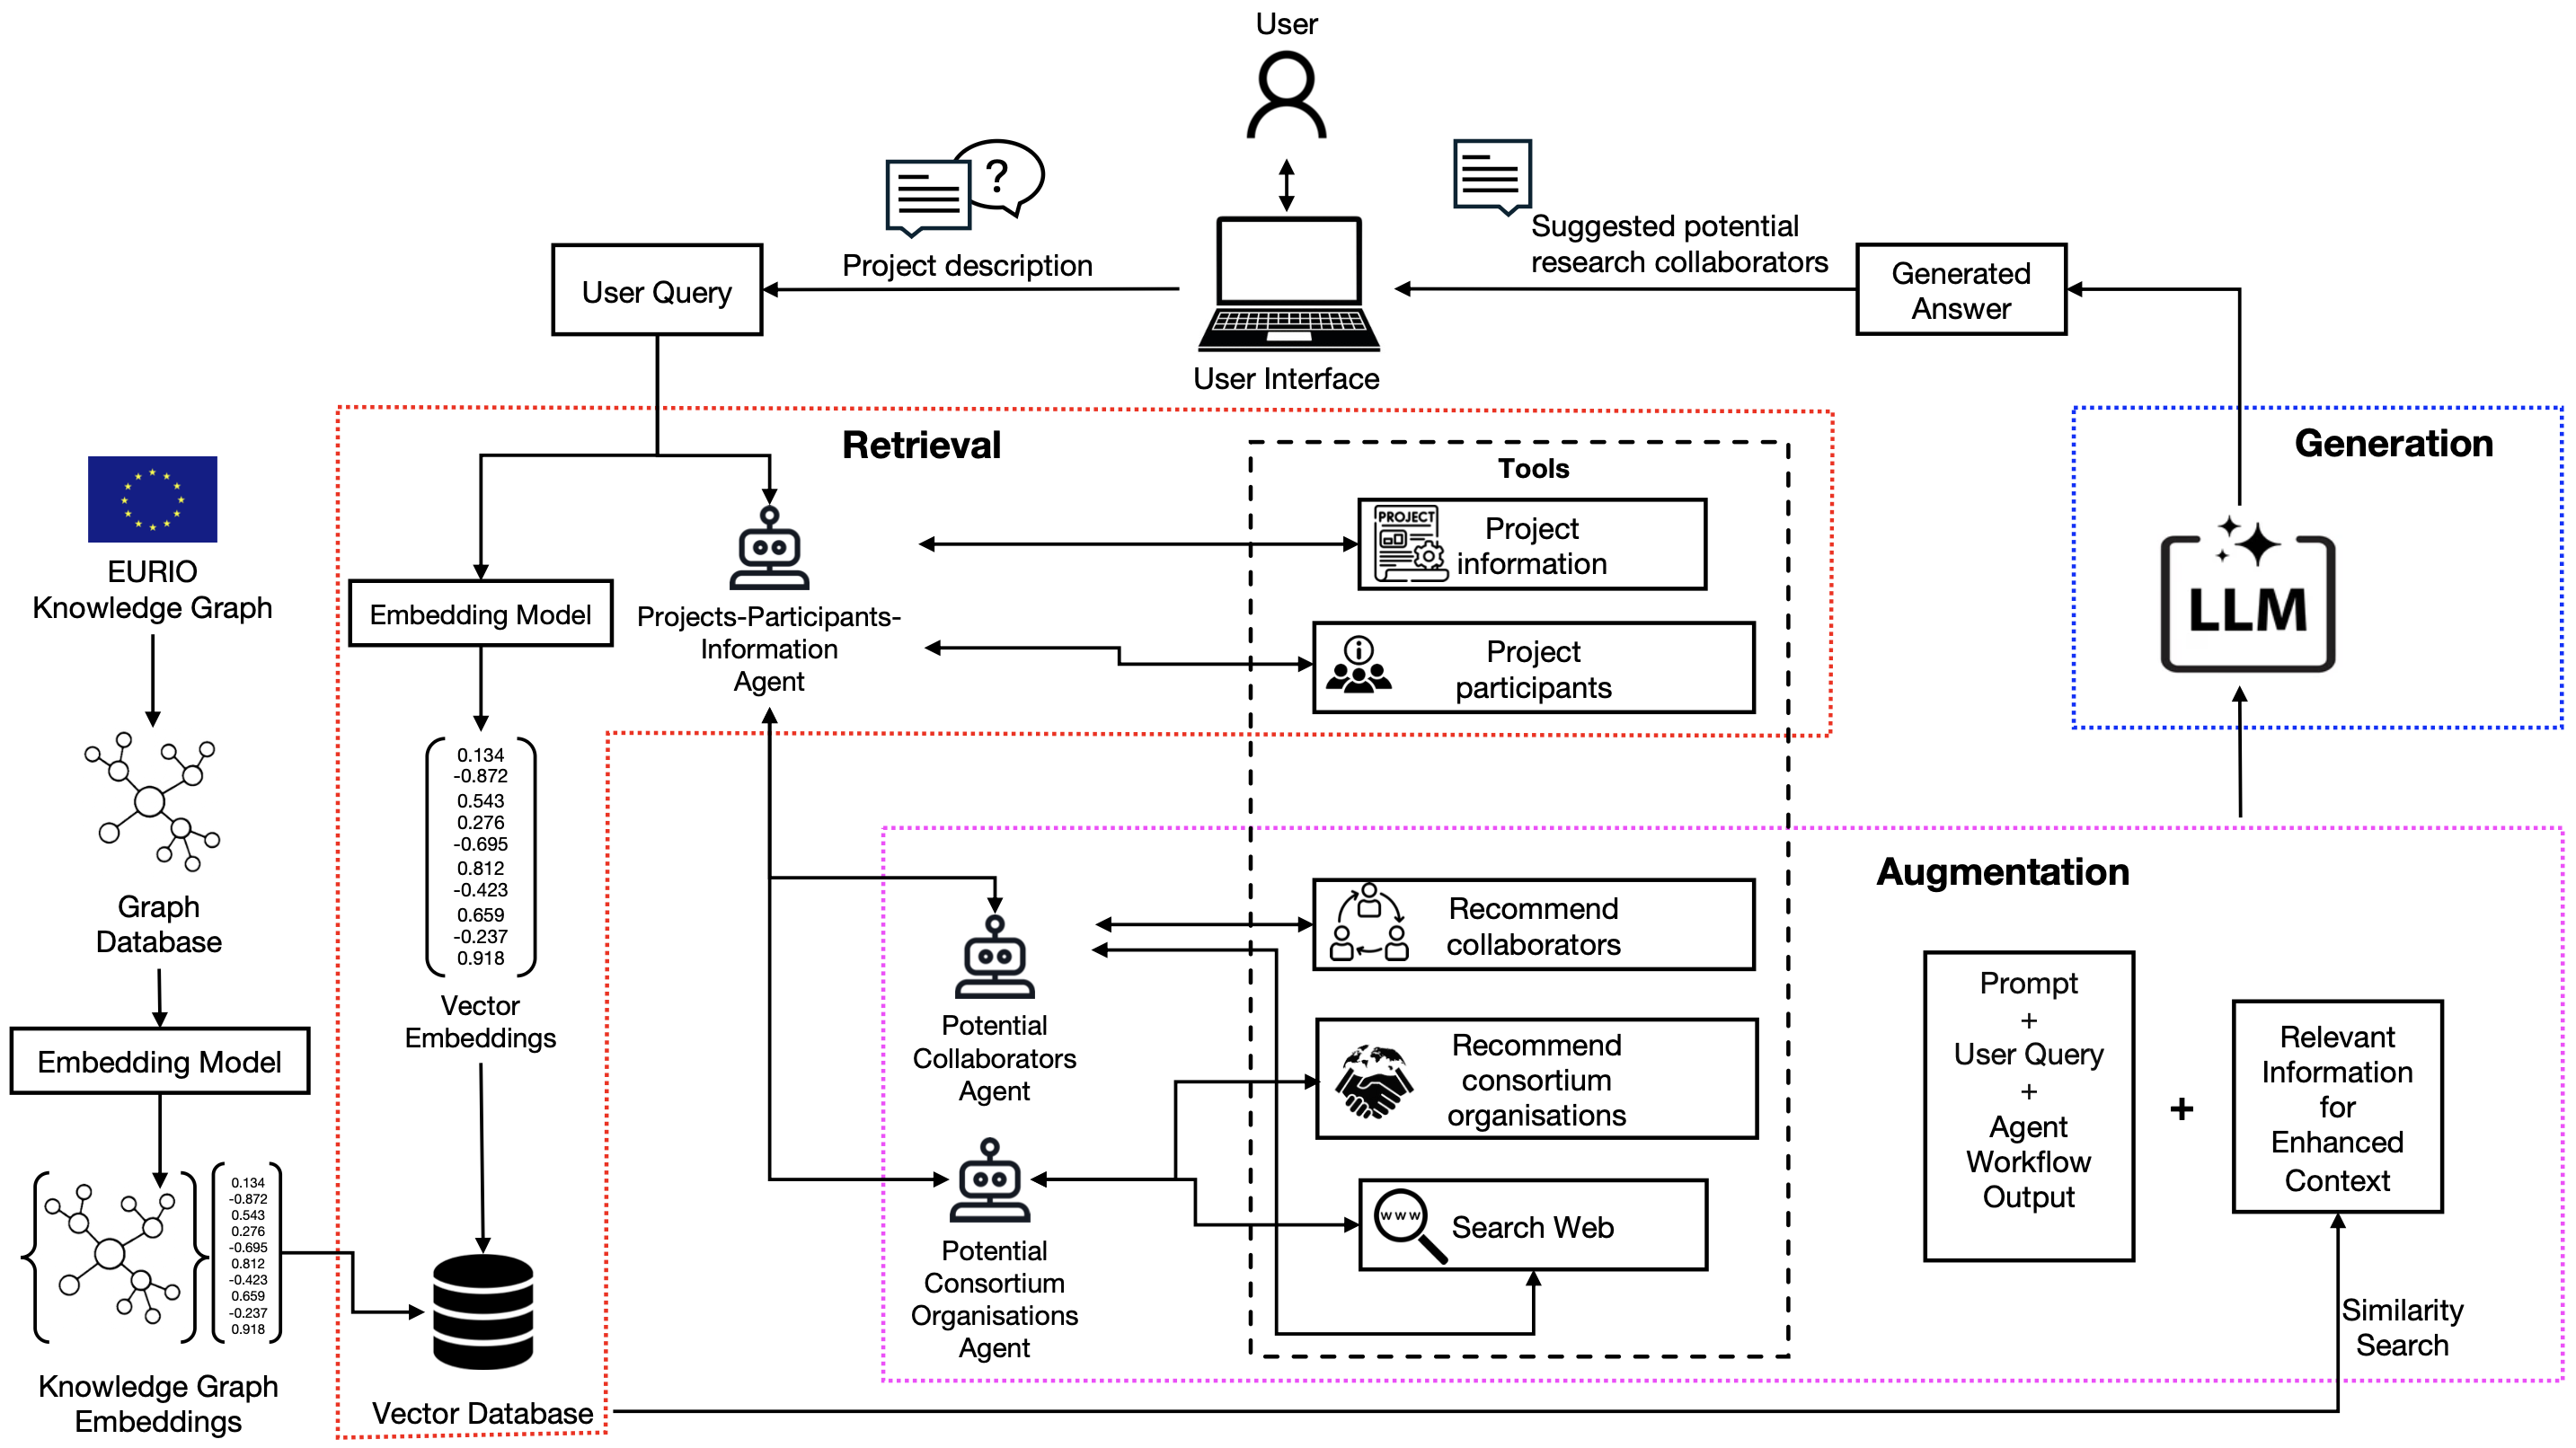
\includegraphics[width=.9\textwidth]{figures/architecture/proposed-system-graphRAG.png}
     \rule{35em}{0.5pt}
    \caption{The proposed Knowledge-Driven and Hybrid AI Architecture for Research Collaboration}
 \label{fig:proposed-system-graphRAG}
\end{figure}

\subsection*{User Interface}
The user interface of the system is designed as a chatbot to provide a user-friendly experience for researchers.
The chatbot provides information retrieval and the two types of recommendations illustrated in Sec.~\ref{sec:recommendation-strategy}.
The user can request information on people, projects and organisation details etc. in the context of European research projects.
It allows users to input a project description and objectives, and receive recommendations for potential research collaborators and consortia.
The interface is designed to be intuitive and easy to use, with clear instructions and guidance on how to input the required information.
The recommendations are displayed in a clear and structured format, with detailed information about each recommended collaborator or consortium, including their expertise, experience, and relevance to the project.

\subsection*{Graph Database}
The \gls{eurio} \gls{kg} is stored as \gls{rdf} format in a graph database, which provides a flexible and efficient way to represent and query the complex relationships between entities in the system.
The graph database allows for the storage of structured data about research projects, organizations, and participants, and enables the retrieval of relevant information based on the relationships between these entities.

\subsection*{Embedding Model and Vector Database}
The embedding model and the vector database play a crucial role in the retrieval process of the proposed system.
\gls{eurio}'s \gls{kg}, stored in a graph database, is transformed through an embedding model, which converts structured information into numerical vector representations.
These embeddings capture the semantic relationships between entities in the \gls{kg}, enabling efficient similarity searches.
The generated vector embeddings are stored in a vector database, facilitating rapid retrieval of relevant knowledge.
When a user submits a query, it is also converted into an embedding and compared against the stored vectors in a similarity search to identify relevant projects, participants, or research entities (satisfied \gls{lr}2).

\subsection*{Agentic Graph Retrieval-Augmented Generation}
Our approach combines the Graph\gls{rag} and Agentic\gls{rag} paradigms to create a hybrid \gls{ai} architecture that leverages the structured data in the \gls{eurio} \gls{kg} and the vector database to generate contextually accurate and consistent recommendations.
According to \cite{singh2025}, modern agents, such as \gls{llm}-powered and mobile agents, are intelligent entities that can perceive their environment, reason about it, and autonomously perform tasks.
In our architecture, 3 agents were defined: the \textit{Project-Participants-Information Agent}, the \textit{Project-Organization-Information Agent}, and the \textit{Project-Researcher-Information Agent}.
These agents follow two agentic workflow patterns \cite{singh2025}: the tool use pattern and the multi-agent collaboration pattern (satisfied \gls{lr}4).
As explained in the following paragraphs, the proposed architecture consists of three main components: Retrieval, Augmentation, and Generation, and agents work together within these components, using external tools to expand their capabilities to achieve specific goals.
A detailed description of each agent using its own tools is given in Sec~\ref{sec:building-ai-agents}.

\paragraph*{Retrieval Component.}
This component is responsible for retrieving relevant information from the \gls{eurio} \gls{kg} and the vector database.
The agent workflow is always initiated by the master agent: the \textit{Project-Participants-Information Agent}.
This agent is responsible for returning information about projects, such as the (e.g. project abstract), and also for returning information about the participants involved in that project (e.g. person full name, organization details).
To perform the retrieval of this information, the agent was specified to follow a template prompt, in which it is instructed to generate \gls{sparql} queries to query the \gls{eurio} \gls{kg} from which to extract data.
Depending on the task to be performed, the master agent will delegate that task to the agent responsible for that task, if necessary.

\paragraph*{Augmentation Component.}
In addition to combining the user query, prompt templates, and information retrieved from the agent master, with all relevant information obtained from the similarity search (satisfied \gls{lr}2), this component adds additional data from the activity performed by the agent workflow.
Cosine similarity was used as a metric for semantic search to determine the similarity of embeddings.
In this component, the agents \textit{Potential Collaborators Agent} and \textit{Potential Consortium Organisations Agent} are responsible for creating the recommendations.
The \textit{Potential Collaborators Agent} has the task of recommending research collaborators, given a project description as input.
The \textit{Potential Consortium Organisations Agent} has the task of creating several consortia formed by various organisations, which contribute to the consortium in a complementary way, i.e. there will be no consortia with organisations specialising in the same research area.
These two agents use the \textit{recommend collaborators} tool, and the \textit{Recommend consortium organisations} tool, respectively, to accomplish the tasks previously described, and they too are instructed with specific prompt templates to follow to achieve their goal.
In addition, both use the \textit{search web} tool, to enrich the information obtained, such as a researcher's areas of interest (satisfied \gls{appr}3), which are not present within the \gls{eurio} \gls{kg}.
In this way, agents act autonomously and are able to make dynamic decisions, resulting in better results than a graph.

\paragraph*{Generation Component.}
Finally, the generation component combines all previously retrieved and augmented information with the pre-trained knowledge of the \gls{llm} to generate contextually accurate and consistent responses.
In addition to providing relevant recommendations, this component ensures explainability by offering detailed justifications for suggested research collaborators, outlining the reasons behind their selection based on expertise, involvement in previous projects and research alignment.
It also describes how the proposed research consortia are composed, specifying the complementary roles of the participating organisations and their collective ability to achieve the project objectives.
This increases transparency and trust in the recommendation process, making the system a valuable tool for making informed decisions in research collaborations.